\section{アンケート調査}\label{アンケート調査}
\ref{Webサイトについて}章で述べるサイトを対象者が閲覧した後の娯楽ゲームの教育的なメリットへの理解とイメージの変化を調査するためにアンケートを行った.

\subsection{調査概要}
調査対象である小中学生の子を持つ保護者10人に調査を行った.
対象者の情報については表\ref{table:情報}に示す対象者の子の年齢や図\ref{fig:ゲーム所持}に示すゲームをプレイする機器の所持状況の他に図\ref{fig:プレイ頻度(回答者)}に示す回答者が週にゲームをプレイする頻度や図\ref{fig:プレイ頻度(子ども)}に示す子が週にゲームをプレイする頻度,図\ref{fig:好き嫌い(回答者)}に示す回答者のゲームの好き嫌い,図\ref{fig:好き嫌い(子ども)}に示す子どものゲームの好き嫌い,図\ref{fig:子どものころ}に示す回答者が子供の頃のゲームプレイの頻度の7項目を収集した.

\begin{table}[H]
 \caption{対象者の子どもの年齢分布}
 \label{table:情報}
 \small
 \centering
  \begin{tabular}{rrrrrrrrr}
  \hline
   子の年齢 & 未就学児 & 小学1,2年 & 3,4年 & 5,6年 & 中学1年 & 2年 & 3年 & 高校以上\\
   (人)& 2 & 3 & 2 & 4 & 3 & 1 & 2 & 0\\
   \hline
  \end{tabular}
\end{table}

\begin{figure}[H]
 \begin{center}
  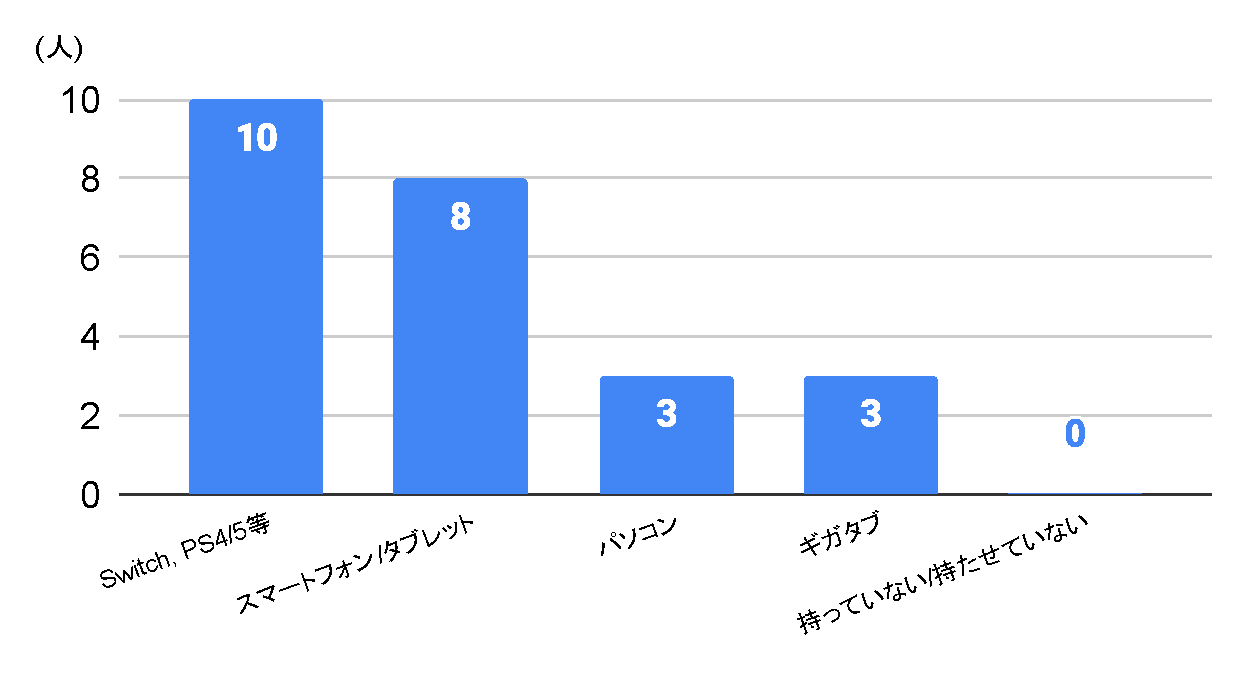
\includegraphics[keepaspectratio, scale=0.6]{PDF/chart1.pdf}
 \end{center}
 \caption{子どもも使用できる家庭用のゲーム機,スマートフォン,タブレット等はあるか}
 \label{fig:ゲーム所持}
\end{figure}

図\ref{fig:ゲーム所持}に示すゲーム機器の所持状況についてはNintendo SwitchやPlayStation4/5といった家庭用ゲーム機やスマートフォン・タブレット端末,またパソコンや学校から配布されたタブレット端末・パソコンであるギガタブを選択肢とした.
子どもの対象が小中学生のためか家庭用ゲーム機が10票,スマートフォン・タブレットが8票と多くを占めた.

\begin{figure}[H]
 \begin{center}
  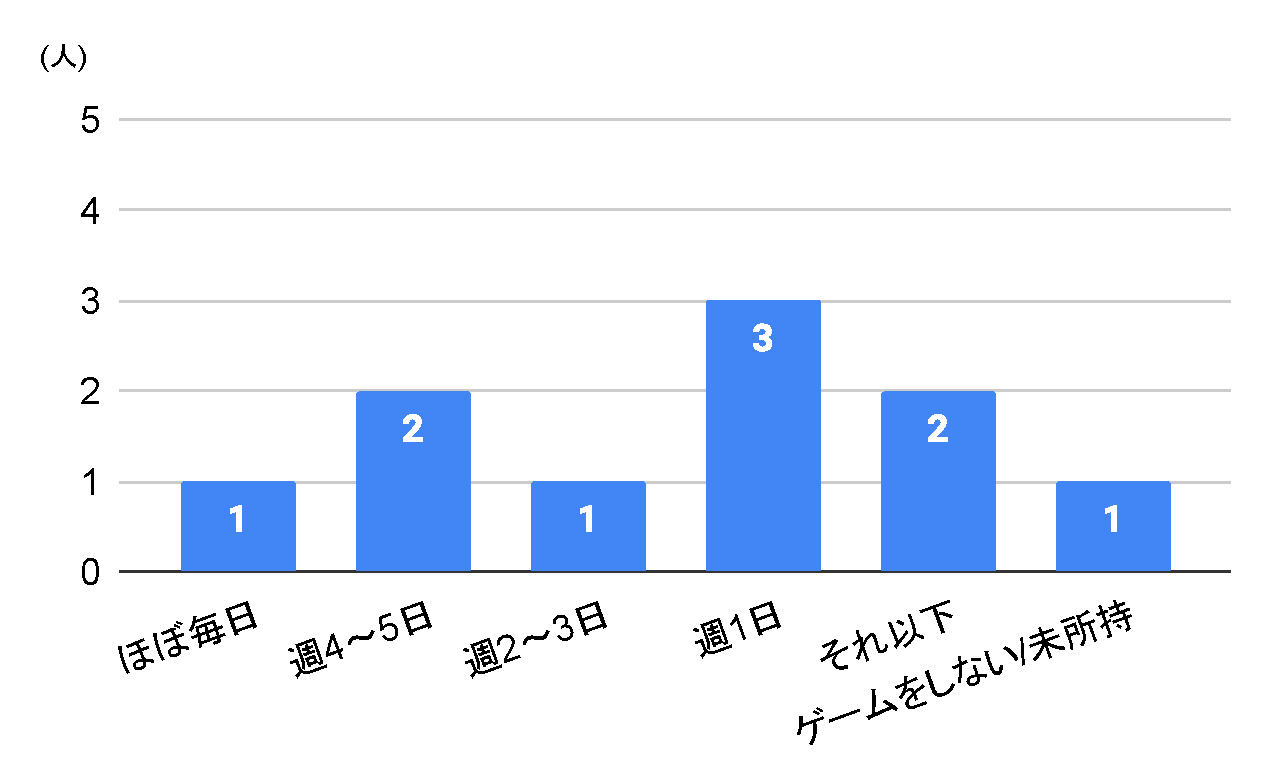
\includegraphics[keepaspectratio, scale=0.6]{PDF/chart2.pdf}
 \end{center}
 \caption{回答者はどれくらいの頻度でゲームをプレイするか}
 \label{fig:プレイ頻度(回答者)}
\end{figure}

\begin{figure}[H]
 \begin{center}
  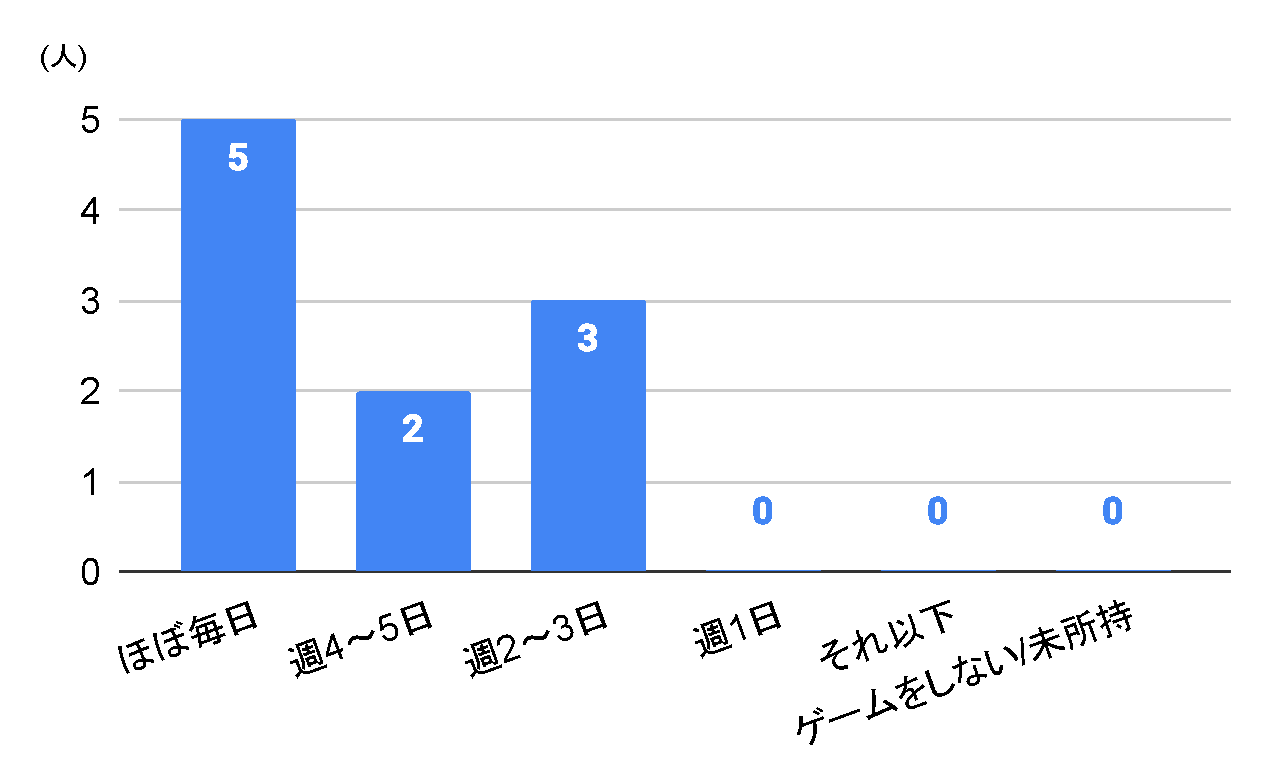
\includegraphics[keepaspectratio, scale=0.6]{PDF/chart3.pdf}
 \end{center}
 \caption{子どもはどれくらいの頻度でゲームをプレイするか}
 \label{fig:プレイ頻度(子ども)}
\end{figure}

図\ref{fig:プレイ頻度(回答者)}と図\ref{fig:プレイ頻度(子ども)}の回答者と子どものゲームのプレイ頻度についての質問では,回答者である保護者は週1日と週4~5日プレイするという人が多く頻度はそれほど高くなかったが,子どものプレイ頻度はほぼ毎日するという人が半数を占めそれ以外も高頻度でプレイしていることが分かった.

\begin{figure}[H]
 \begin{center}
  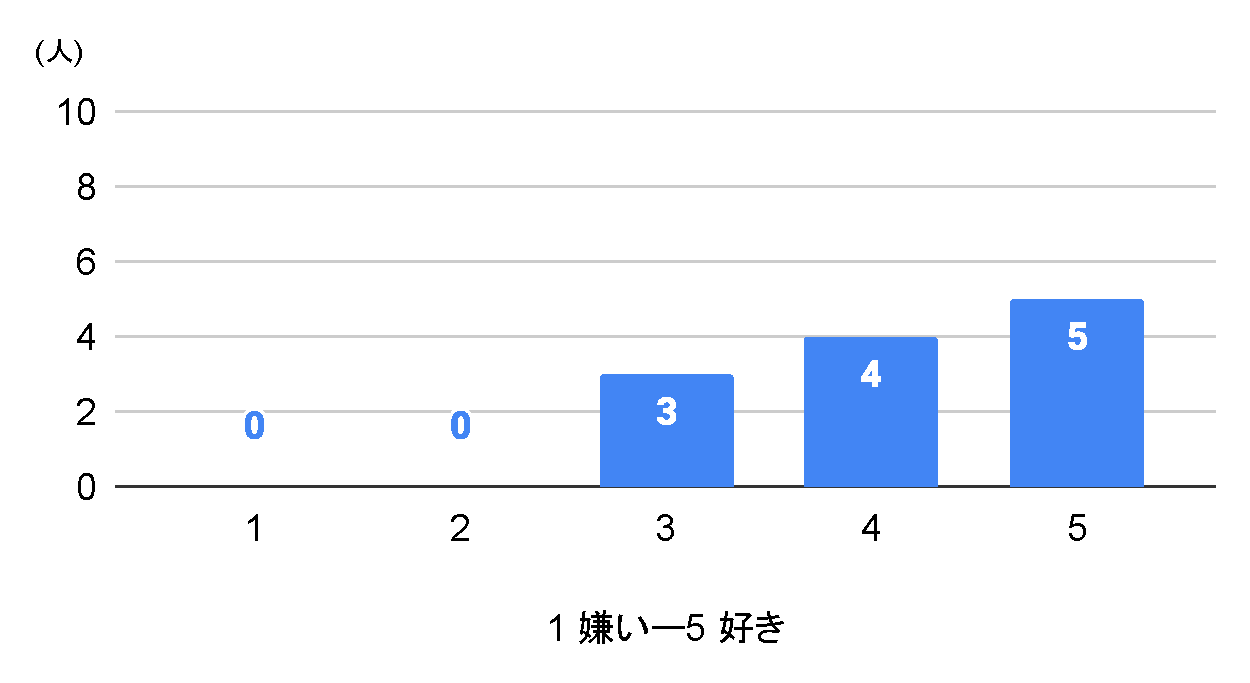
\includegraphics[keepaspectratio, scale=0.6]{PDF/chart4.pdf}
 \end{center}
 \caption{回答者はゲームが好きか}
 \label{fig:好き嫌い(回答者)}
\end{figure}

\begin{figure}[H]
 \begin{center}
  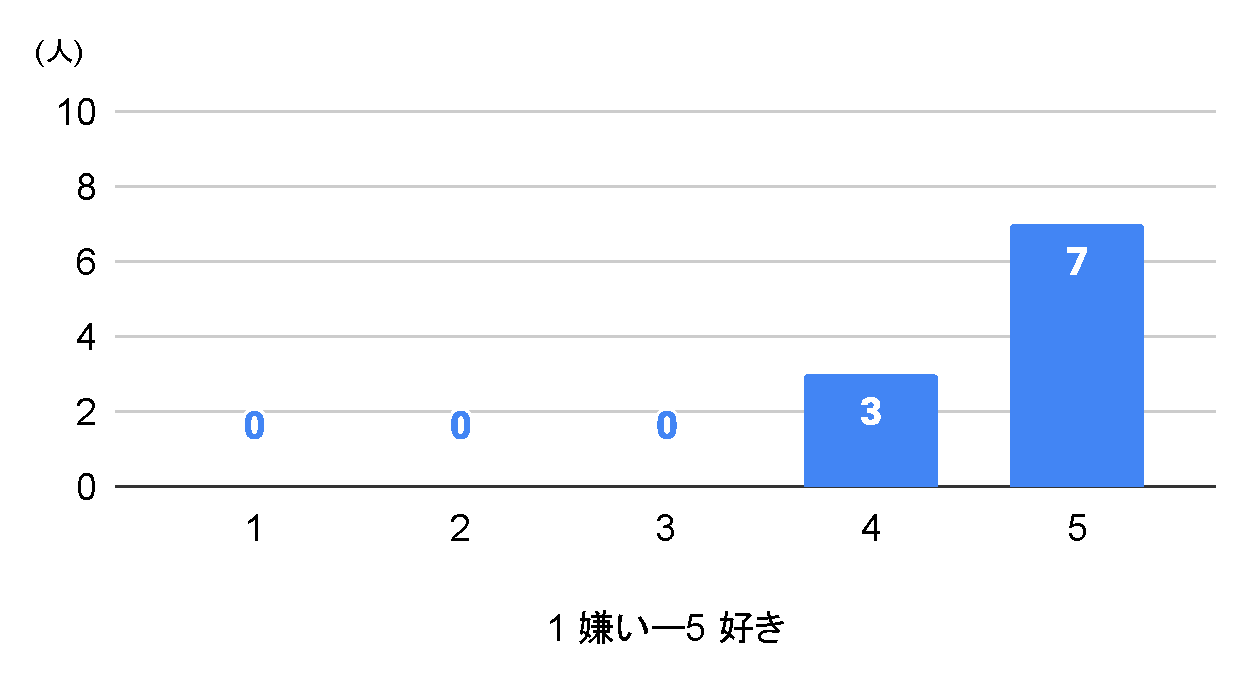
\includegraphics[keepaspectratio, scale=0.6]{PDF/chart5.pdf}
 \end{center}
 \caption{子どもはゲームが好きか}
 \label{fig:好き嫌い(子ども)}
\end{figure}

図\ref{fig:好き嫌い(回答者)}の回答者はゲームが好きかという質問では回答者である保護者は嫌いという回答はなくどちらでもないから好きである傾向にあった.
図\ref{fig:プレイ頻度(回答者)}の回答者のプレイ頻度ではあまりゲームをしないという人もいたが,ゲームが嫌いという傾向にないことが分かった.
これは図\ref{fig:子どものころ}の回答者が子どもの頃ゲームで遊ぶことがあったかという質問の回答からよくプレイしたという人が多かったためだと考えられる.

図\ref{fig:好き嫌い(子ども)}の子どもはゲームが好きかという質問ではやや好きが3票,好きが7票という結果になった.
図\ref{fig:プレイ頻度(子ども)}の子どものゲームのプレイ頻度の傾向から見てもゲームが好きである人が多いことは容易に窺える.

\begin{figure}[H]
 \begin{center}
  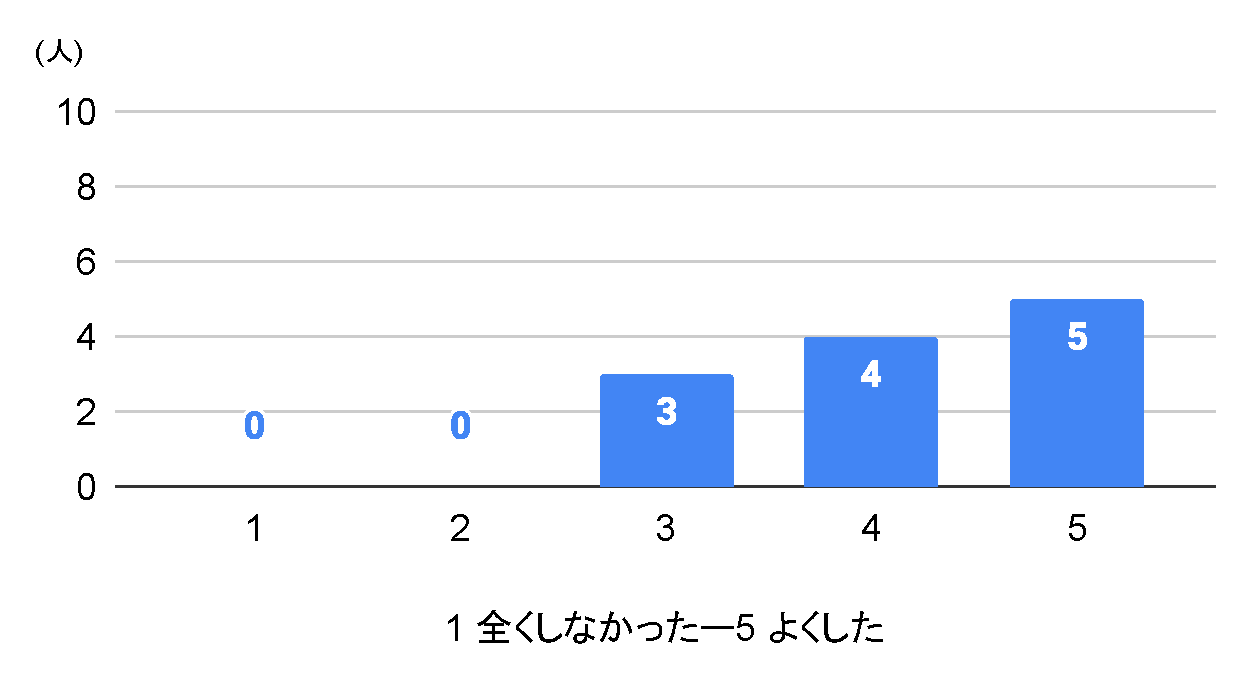
\includegraphics[keepaspectratio, scale=0.6]{PDF/chart6.pdf}
 \end{center}
 \caption{子どもの頃ゲームで遊ぶことはあったか}
 \label{fig:子どものころ}
\end{figure}

\subsection{調査項目}\label{調査項目}
調査として表\ref{table:anque}に示すように回答者にゲームが子どもに与える影響について全体的にどのようなイメージを持っているかを聞き,さらにその詳細としてi.勉強面,ⅱ.友人関係・コミュニケーション,ⅲ.感性,ⅳ.知識・教養,v.時間管理,ⅵ.健康面の影響についてのイメージと読書やⅶ.スポーツといった他の趣味活動とのメリットの比較を,Webサイトを見る前と見た後について全17問調査した.
項目については株式会社アスマークが行ったアンケート調査\cite{gameanq}の表\ref{table:asmarqanque}の意見記述の一部を参考に,iはa,b,ⅱはc,d,ⅲはe,ⅳはd,vはb,f,ⅵはg,ⅶはhと対応するようにゲームが子どもにとって良い悪いに関わらず影響を与えると考えられているもの7個を扱った.

さらにアンケートの最後部に,作成した記事に書かれたゲームについてのメリットが今後の子どもの発育・成長に影響があると思うかという質問と意見記述の欄を設けた.

\begin{table}[H]
 \caption{アンケート項目}
 \label{table:anque}
 \small
 \centering
  \begin{tabular}{l}
  \hline
  子に与える影響について \\
   \hline
    i.勉強面 \\
   ⅱ.友人関係,コミュニケーション\\
   ⅲ.感性\\
   ⅳ.知識,教養 \\
    v.時間管理   \\
   ⅵ.健康面 \\
   ⅶ.読書・スポーツ等他の趣味とのメリットの比較 \\
   \hline
  \end{tabular}
\end{table}


\begin{table}[H]
 \caption{アスマークによるアンケート調査の意見記述(一部抜粋)}
 \label{table:asmarqanque}
 \small
 \centering
  \begin{tabular}{l}
  \hline
   a. 最近では勉強できるソフトもたくさんあって,自分自身役に立っている\\
   b. 学習時間や運動の時間,睡眠時間を削ることにつながる \\
   c. 現実から逃避され,人とのコミュニケーションがなくなる \\
   d. 友人関係の形成,コミュニケーションツール,知識の習得と言った面ではプラスの作用もある \\
   e. 感性が豊かになるとは思うが,結局はムダな時間ではあるのでバランスが大事だとは思う \\
   f. 遊ぶ時間などのルールをきっちりと決め,親の管理の上でやらせなければ無制限にやることになる\\
   g. 外で身体を動かす遊びを全くしなくなった.動かないので太りやすい \\
   h. 読書して知識や想像力を蓄えたほうが良い \\
   \hline
  \end{tabular}
\end{table}
